%!TEX root = planning.tex
\section{Tasks \& Schedule}

The main tasks of this project are the following:
\begin{enumerate}
    \item Creation of the \textbf{Requirement Analysis and Specification Document} \cite{bib:rasd}, which explains in detail functional and nonfunctional requirements, domain assumption and goals of the application to be built.
    \item Creation of the \textbf{Design Document} \cite{bib:dd}, which deals with the architecture and the design shape of the application.
    \item Creation of the \textbf{Integration Testing Plan Document} \cite{bib:itpd}, which contains integration testing strategy we intend to apply to the application.
    \item Creation of the \textbf{Project Plan}, this document.
    \item Preparation of a quick \textbf{presentation}, using slides, ($\sim 10$ min) of the previously mentioned documents to our client.
    \item \textbf{Development} of the entire application and the preparation of the unit tests.
    \item Running of \textbf{integration testing} on the application.
\end{enumerate}

For the first tasks the activities were already given along with corresponding deadlines for the submission of needed documents. Starting from the implementation, instead, no schedule was given so, according to the COCOMO estimation performed and described in \ref{sec:cocomo} QUI VA LA DATA DI TERMINE PER SVILUPPO + TESTING. % TODO!!!

The development of the application started after the creation of the Design Document and will be carried on in parallel with the rest of the tasks.
After the completion of the ITPD, tests will be run on the developing application in order to verify the proper functioning of every new functionality added.

In~\autoref{fig:tasks-dep-graph} you can find the dependency graph of every task, in~\autoref{tab:schedule}, instead, you can find the schedule of every task. Also the Gantt chart for the project is provided in~\autoref{fig:gantt}.


\begin{figure}
    \centering
    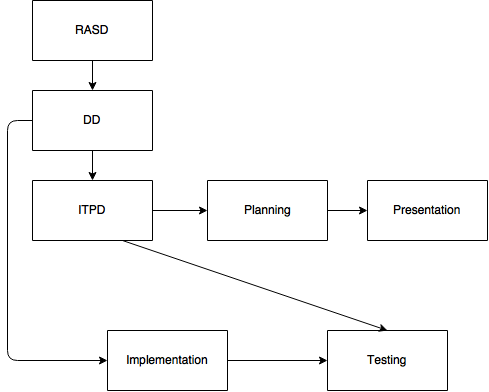
\includegraphics[width=\textwidth]{img/tasks-dep-graph.jpg}
    \caption{Dependencies between tasks shown as graph.}
    \label{fig:tasks-dep-graph}
\end{figure}

\begin{table}[p]
    \centering
    \begin{tabular}{| l | l | l |}
        \hline
        \textbf{Activity}   & \textbf{Start Date}   & \textbf{Deadline} \\
        \hline
        RASD                & 2015-10-15            & 2015-11-06        \\
        DD                  & 2015-11-11            & 2015-12-04        \\
        ITPD                & 2016-01-07            & 2016-01-21        \\
        Project Plan        & 2016-01-21            & 2016-02-02        \\
        Presentation        & 2016-02-02            & 2016-02-12        \\
        Implementation      & 2015-12-05            & DA DEFINIRE       \\
        Integration Testing & 2016-01-22            & DA DEFINIRE       \\
        \hline
    \end{tabular}
    \caption{Schedule for project tasks.}
    \label{tab:schedule}
\end{table}

\begin{figure}[p]
    \hspace*{-1.5cm}
    \begin{ganttchart}[
        vgrid={*{6}{draw=none},dotted},
        time slot format=isodate,
        x unit=0.7mm,
        today=2016-02-02,
        today rule/.style= {blue, ultra thick},
        today label=Today,
        link bulge=6, link tolerance=5,
        bar inline label node/.style={font=\scriptsize},
        inline
        ]{2015-10-10}{2016-06-20}
        \gantttitlecalendar{year, month} \\
        \ganttbar[name=rasd]{RASD}{2015-10-15}{2015-11-06} \\
        \ganttbar[name=dd]{DD}{2015-11-11}{2015-12-04} \\
        \ganttbar[name=itpd]{ITPD}{2016-01-07}{2016-01-21} \\
        \ganttbar[name=pplan]{Plan}{2016-01-21}{2016-02-02} \\
        \ganttbar[name=pres]{Present.}{2016-02-02}{2016-02-12} \\
        \ganttbar[name=impl]{Implementation}{2015-12-05}{2016-06-01} \\ %Cambiare data fine
        \ganttbar[name=int-test]{IntTest}{2016-01-22}{2016-06-15} %cambiare data fine
        \ganttlink{rasd}{dd}
        \ganttlink{dd}{itpd}
        \ganttlink{impl}{int-test}
    \end{ganttchart}
    \hspace*{-1.5cm}
    \caption{Gantt chart of the project.}
    \label{fig:gantt}
\end{figure}
